\section{Method}\label{sec:method}

In this section we describe the high-level architecture of the system.
The system comprises a variety of off-the-shelf components.  We
describe each component and its configuration.  The components are
loosely coupled and interchangeable.  For example, even though our
system relies on Microsoft Active Directory, any directory service
with dynamic groups and LDAP support will suffice.

\subsection{High-Level Architecture}

The system integrates an access control system for a building with a
directory service such as Microsoft Active Directory.  The access
control system is simulated using a Raspberry Pi and an RFID door
entry system.  When a user enters the building, they swipe their
access card.  This triggers a Python script on the Raspberry Pi that
changes the user's group from an external group to an internal group.
This signifies that they are physically located within the building.
When a user leaves the building, they swipe their access card.  This
triggers the same Python script to change the user's group from the
internal group back to the external group.  This signifies that the
user is physically located outside of the building.  The Web resource
is served by a Web server behind a reverse proxy and load balancer
(Progress Kemp LoadMaster).  This directs the traffic based on the
user's group.  It verifies that the source of the user's connection
matches their known location.  Finally, all of the components send
logs to a Security Information and Event Management (SIEM) service.
This aggregates logs, alerts and events into a centralised service
allowing investigators to perform historical and near real-time
analysis.

The system is novel in at least two aspects.  Firstly, the access
control system dynamically changes a user's group membership in the
directory service based on their physical location.  The rules for the
dynamic groups can be easily combined with existing rules.  Secondly,
the reverse proxy and load balancer direct traffic based on the user's
current group membership.  In this way, the physical location of the
user determines whether the Web resource is accessible or not.

\subsection{The Components}

Our system comprises a variety of off-the-shelf components:

\begin{itemize}
\item Microsoft Active Directory with LDAP support
\item Raspberry Pi connected to an RFID door entry system (see
  Fig.~\ref{fig:raspberry-pi-rfid})
\item Progress Kemp LoadMaster~\cite{progress-kemp-loadmaster-xx}
\item Progress WhatsUp Gold~\cite{progress-kemp-whatsup-gold-xx}
\item Web servers (Apache HTTP Server)
\end{itemize}

We describe each component and its configuration in the following
subsections.

\subsubsection{Microsoft Active Directory With LDAP Support}

\begin{figure}
  \centerline{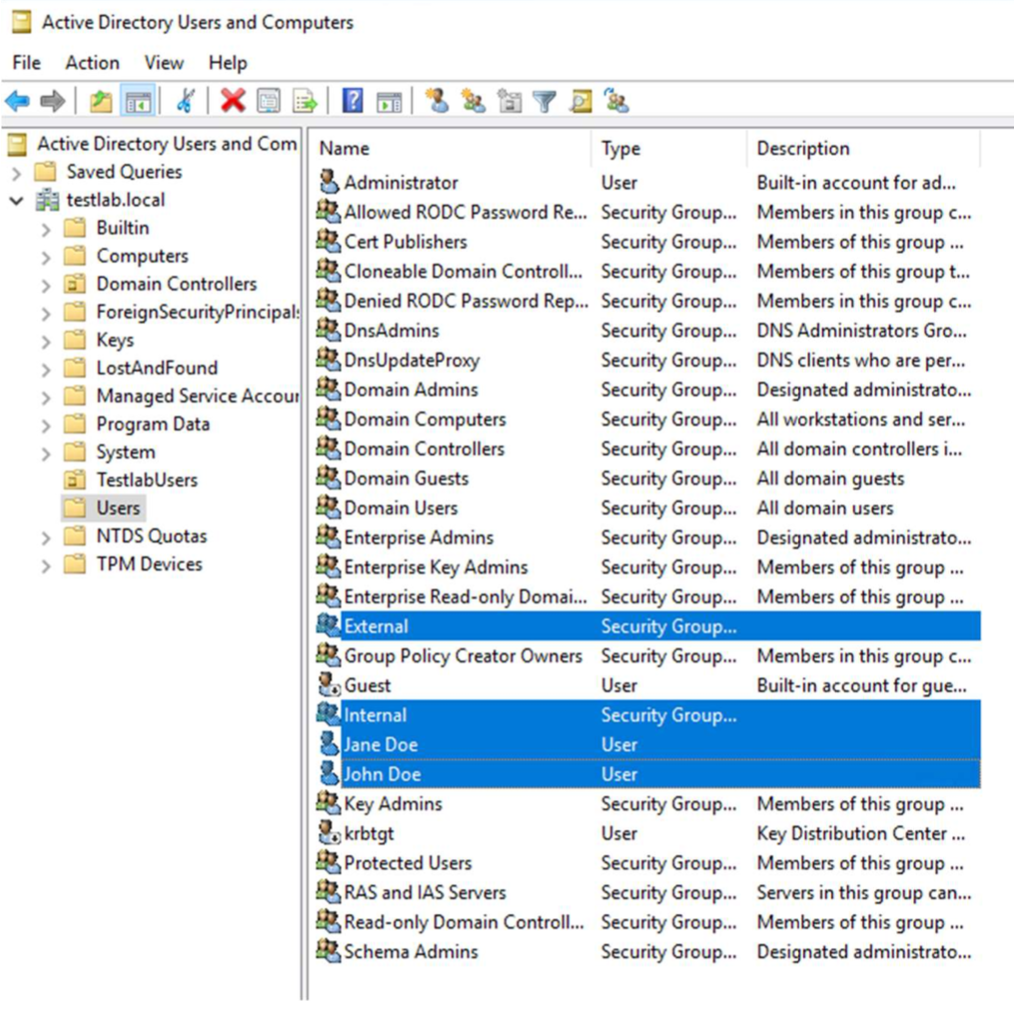
\includegraphics[width=\columnwidth]{img/active-directory}}
  \caption{We created two users, Jane Doe and John Doe, and two
    groups, Internal and External, in Microsoft Active Directory.  We
    also enabled LDAP support.}\label{fig:active-directory}
\end{figure}

We used Microsoft Windows Server 2019 to run a Domain Controller (DC)
(\texttt{d1.testlab.local}) for our domain (\texttt{testlab.local}).
This is the primary DC for the scenario and it was setup to host
Active Directory (AD) with LDAP support and the Domain Name System
(DNS).  AD provides authentication and authorisation services, and
allows administrators to manage network resources centrally.  To
ensure that the requests for the Web resources go to the appropriate
services on the Progress Kemp LoadMaster, we created corresponding DNS
delegations.  This is important as we wanted the external requests to
be pointed to the external resources and the internal requests to be
pointed to the internal resources.  It also allows the LoadMaster to
perform service health checks before responding to DNS requests thus
preventing IP addresses being returned when resources are unavailable.
We added two users, Jane Doe and John Doe, and two groups, Internal
and External, to AD (see Fig.~\ref{fig:active-directory}).

\subsubsection{Raspberry Pi and RFID Door Entry System}

\begin{figure}
  \centerline{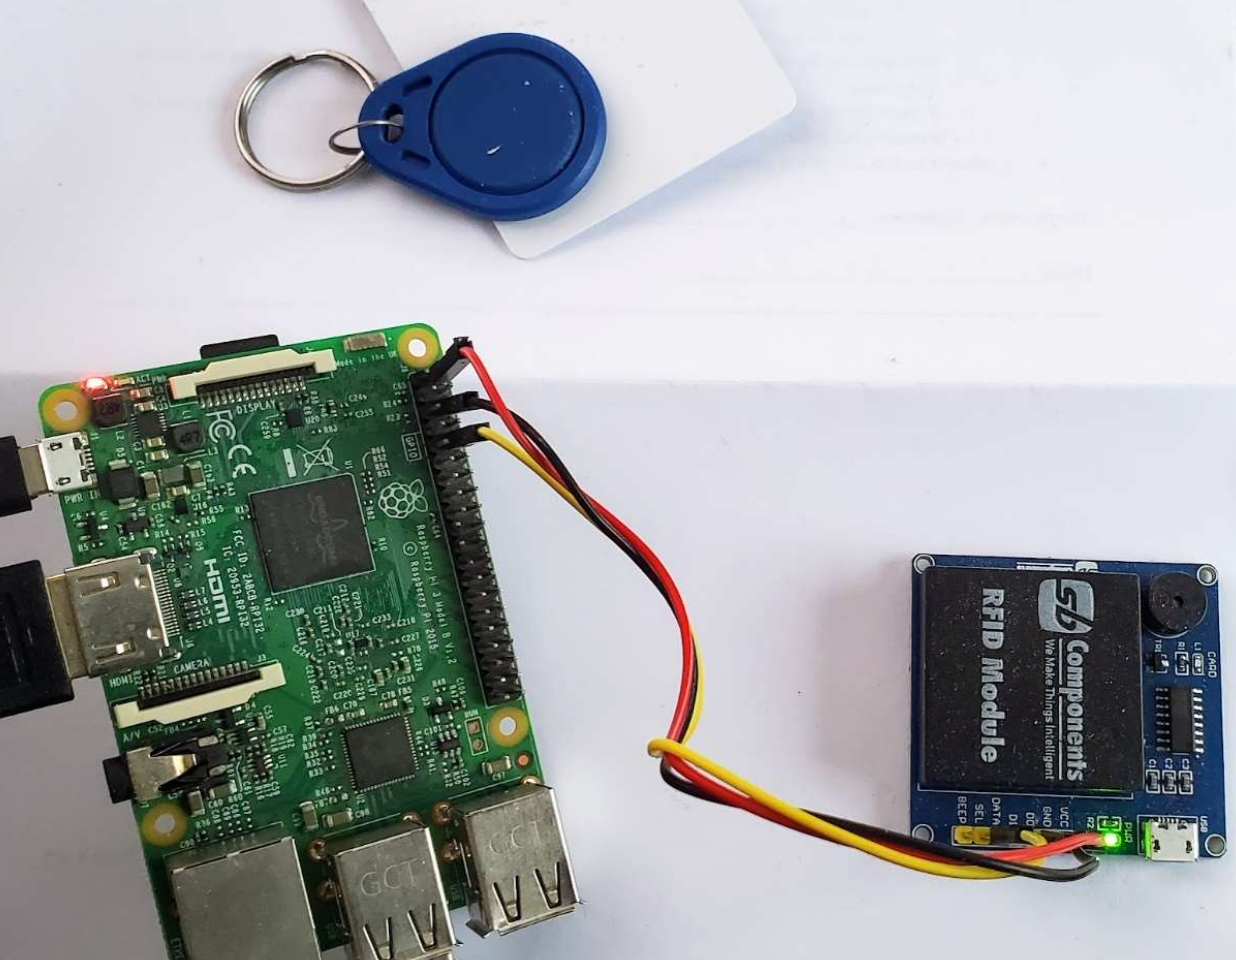
\includegraphics[width=\columnwidth]{img/raspberry-pi-rfid}}
  \caption{The Raspberry Pi was connected to an RFID door entry
    system.  We created a Python script that read the identification
    details from swiped cards and interacted with Active
    Directory.}\label{fig:raspberry-pi-rfid}
\end{figure}

The Raspberry Pi is connected to an RFID door entry system.  When a
user performs a card swipe, a Python script running on the Raspberry
Pi reads the identification details from the card and remotely changes
the group membership of the user in AD.\@ If the user is entering the
building their group membership is changed from External to Internal;
if they are leaving the building it is changed from Internal to
External.  The Python script uses the
\texttt{ldap3}\footnote{https://ldap3.readthedocs.io/} package to
interact with AD.\@ It logs all events to a SIEM service (see
Sect.~\ref{sec:wug}).

\subsubsection{Progress Kemp LoadMaster}

Progress Kemp LoadMaster (LM) is a reverse proxy and load
balancer~\cite{progress-kemp-loadmaster-xx}.  It has many capabilities
but for this scenario we are interested in the Edge Security Pack
(ESP), the source IP blacklist from the GEO component, and the Web
Application Firewall (WAF).  We use the ESP for Single Sign-On (SSO)
for HTTPS services and to communicate with AD during login and to
query group memberships.  This pre-authenticates a user before they
gain access to a resource.  We also enabled \textit{group steering} on
the ESP:\@ this allows LM to send traffic to particular services based
on their group membership in AD and goes beyond the normal use of
groups to simply allow or deny access.

\begin{figure*}
  \centerline{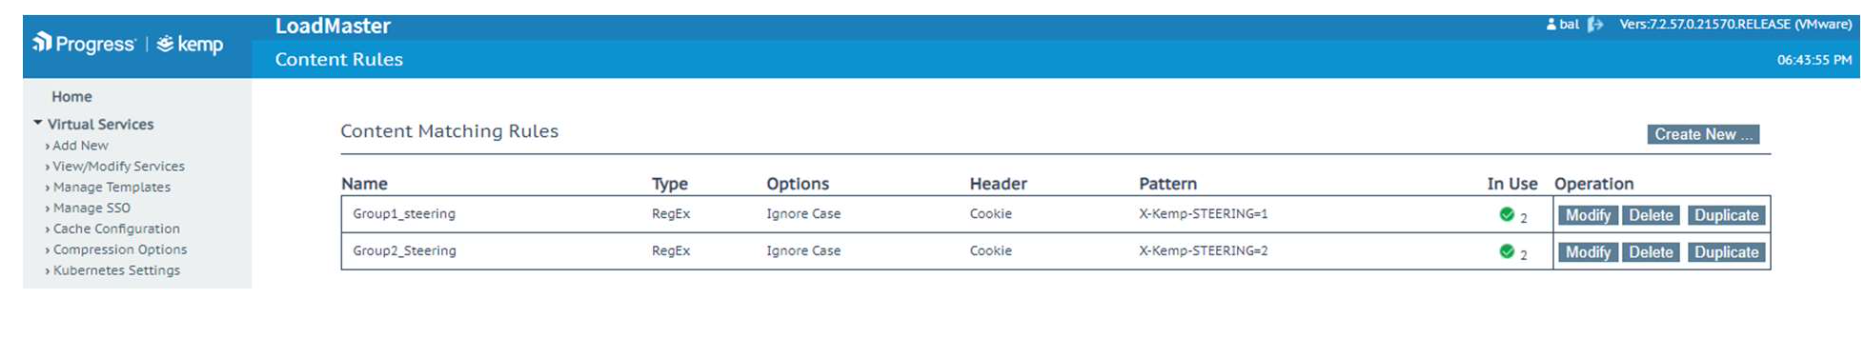
\includegraphics[width=\textwidth]{img/loadmaster-pcre-rules}}
  \caption{LoadMaster can direct traffic based on steering groups: we
    created two such groups, one for internal traffic and one for
    external traffic.}\label{fig:loadmaster-pcre-rules}
\end{figure*}

We created two steering groups associated with the Internal and
External groups in AD.\@ We created Perl Compatible Regular Expression
(PCRE) rules to match the authorisation headers and steer the requests
to the appropriate services (see
Fig.~\ref{fig:loadmaster-pcre-rules}).

The login page that is displayed by the ESP is the same for both
\textit{valid} and \textit{invalid} access attempts.  A valid access
attempt occurs when a user's group and request are both internal or
both external; otherwise the access attempt is invalid.  In both cases
a log is sent to a SIEM service (see Sect.~\ref{sec:wug}).  This helps
with threat hunting as a threat actor will see the same login page for
the honeypot as for the valid site.  The honeypot can gather the
details of the access attempt without being discovered.

\begin{figure*}
  \centerline{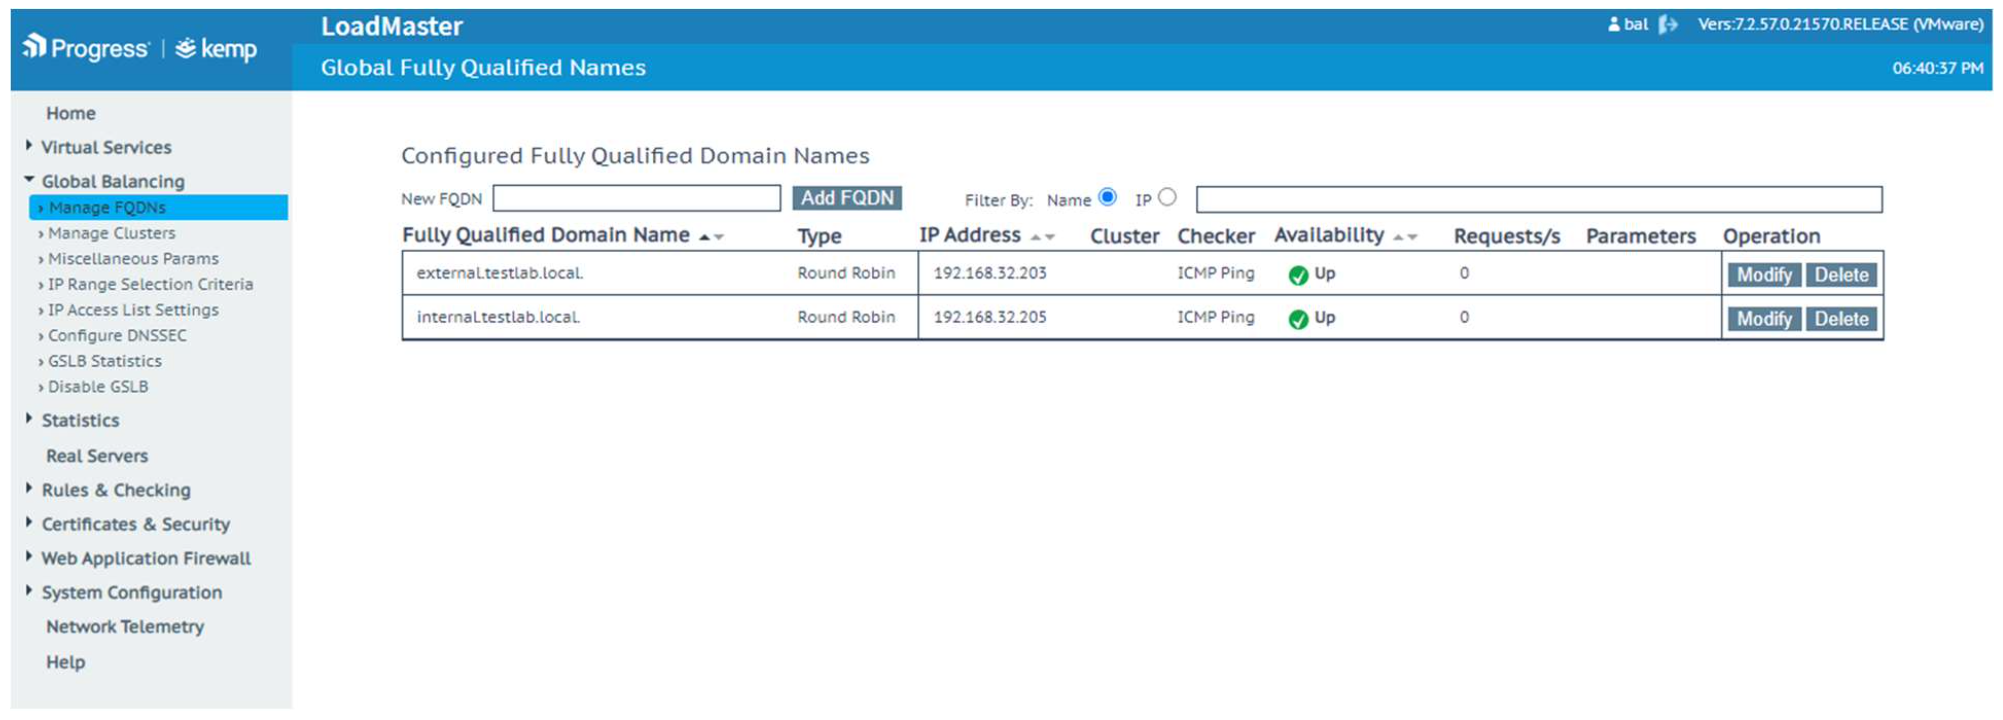
\includegraphics[width=\textwidth]{img/loadmaster-geo}}
  \caption{We configured two FQDNs for \texttt{internal.testlab.local}
    and \texttt{external.testlab.local} using LoadMaster's GEO
    component.}\label{fig:loadmaster-geo}
\end{figure*}

The GEO component performs DNS resolution and service health checks
before returning a result.  We created GEO DNS entries for
\texttt{internal.testlab.local} and \texttt{external.testlab.local}
(see Fig.~\ref{fig:loadmaster-geo}).  We also used an IP blacklist
that is updated daily to withhold DNS results from anyone on the list.

\begin{figure*}
  \centerline{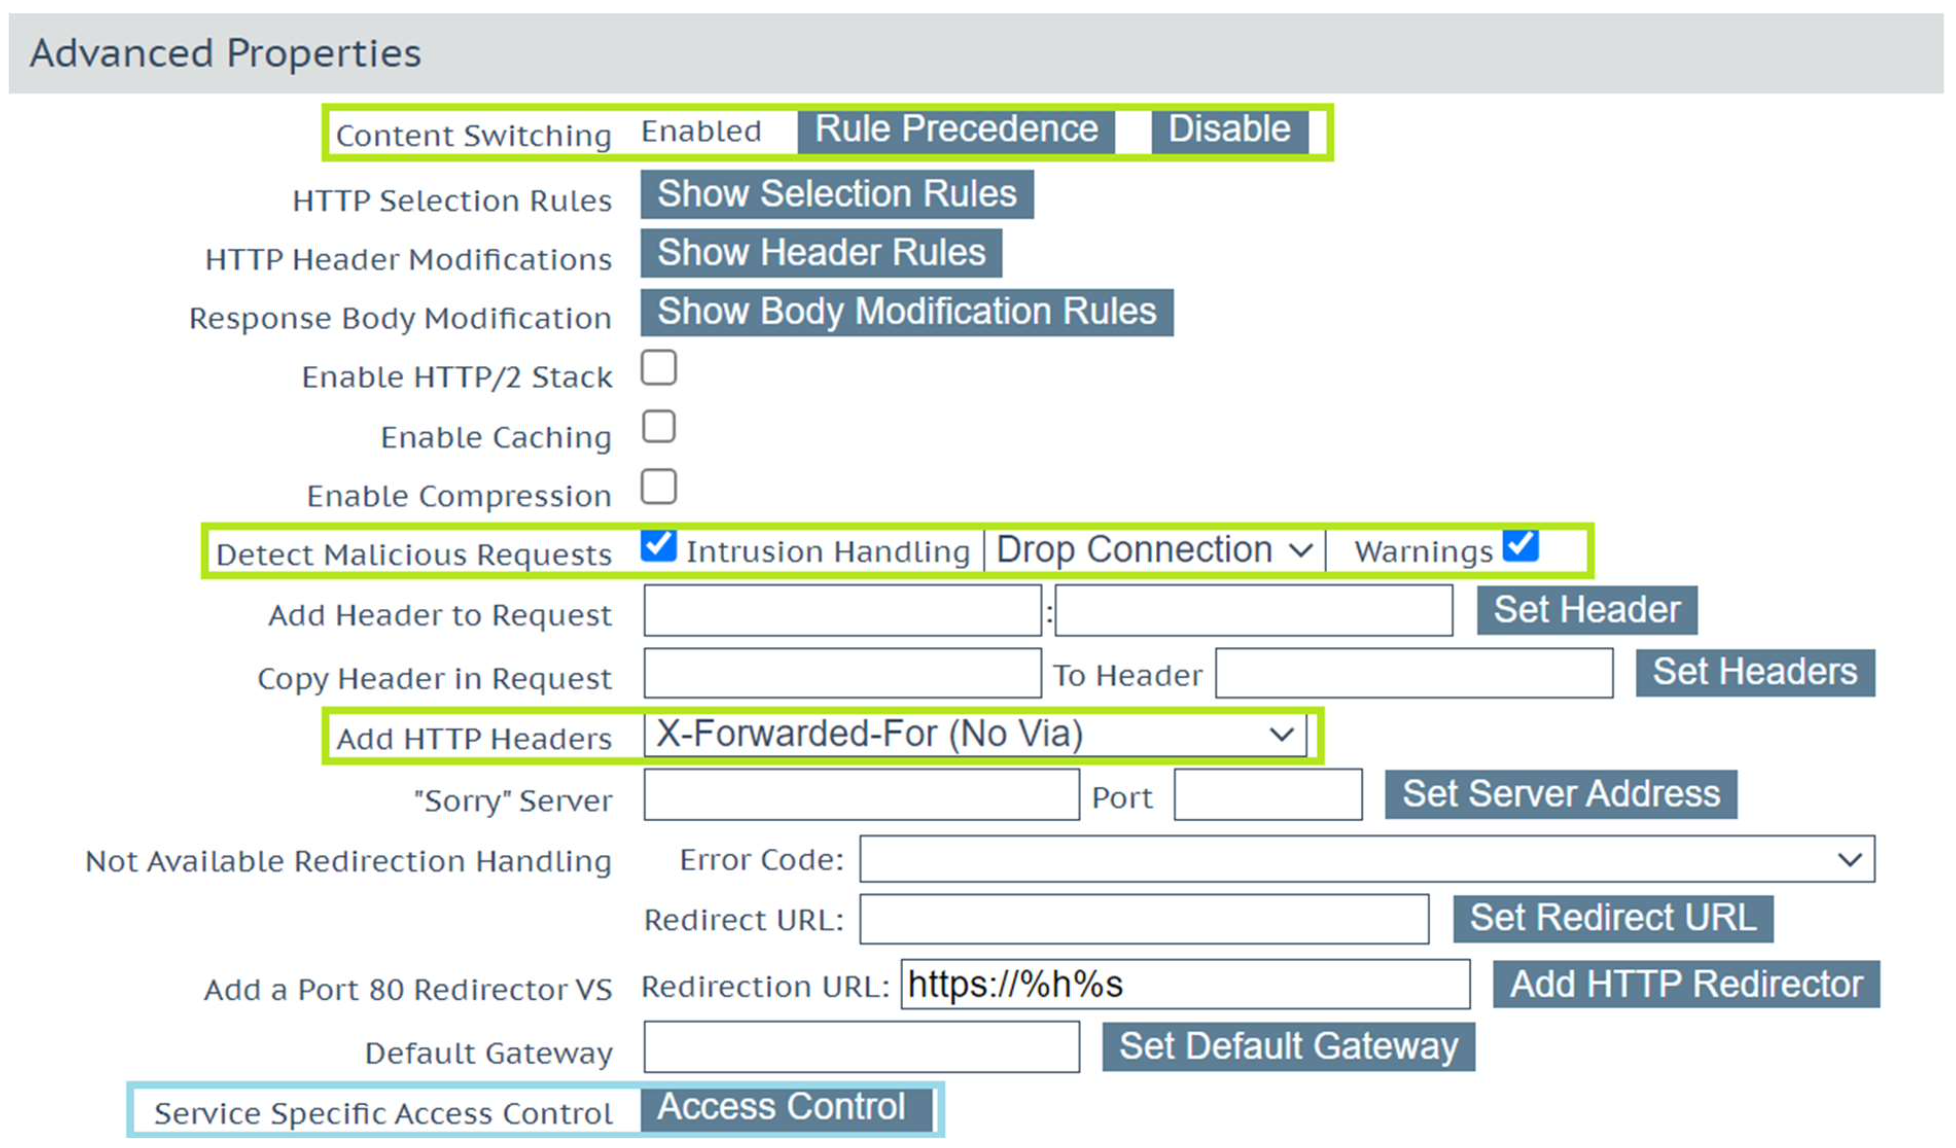
\includegraphics[width=\textwidth]{img/loadmaster-ids-ips}}
  \caption{We enabled Content Switching in LoadMaster so that the PCRE
    engine is enabled for group steering (first green rectangle).  We
    enabled IDS/IPS as an additional layer of defence (second green
    rectangle).  We also added \texttt{X-Forwarded-For} HTTP headers
    to enable the Flask application (honeypot) to easily record the
    originating IP addresses of invalid access attempts (third green
    rectangle).  We could also enable the Service Specific Access
    Control to prevent access via whitelists and blacklists (blue
    rectangle).  This was not enabled during our
    tests.}\label{fig:loadmaster-ids-ips}
\end{figure*}

Additionally, we enabled the Intrusion Detection System (IDS) and
Intrusion Prevention Systems (IPS) on LM.\@ This includes rules
defined by the Snort community~\cite{cisco-snort-xx} and enables the
Snort rule filtering on the Layer 7 HTTP engine to check for any known
bad requests.  Figure~\ref{fig:loadmaster-ids-ips} shows the
configuration highlighted in green.  There is also an option to
prevent access via whitelists and blacklists highlighted in blue.

Finally, we enabled the Web Application Firewall (WAF) and the Open
Web Application Security Project (OWASP) core rule set.  This rule set
performs anomaly scoring and identifies, for each request, the
probability that it is malicious.  The core rule set protects against
SQL injection, cross-site scripting, remote code execution, buffer
overflows, known vulnerabilities, and many other attack vectors.  We
configured the WAF with source IP reputation blocking enabled which
uses a global IP reputation list that is updated daily.  Using the
MaxMind~\cite{maxmind-xx} and the GEO component, it identifies the
country of the source request and it can be configured to block
specific countries or regions.

\subsubsection{Web Servers}

Our Web servers are hosted on virtual machines running Debian and a
default installation of the Apache HTTP Server.  The landing page is
our ``valid access'' page and represents our secured Web resource.
The ``invalid access'' page is served by a Flask
application\footnote{https://flask.palletsprojects.com/}.  It records
the usernames and source IP addresses of all requests and sends those
details to a SIEM service (see next section).  The details are
extracted from the authorisation and \texttt{X-Forwarded-For} headers.
The Flask application is a honeypot: it reports to a user that a
requested resource is unavailable rather than reporting that an access
attempt was invalid.

\subsubsection{Progress WhatsUp Gold}\label{sec:wug}

\begin{figure*}
  \centerline{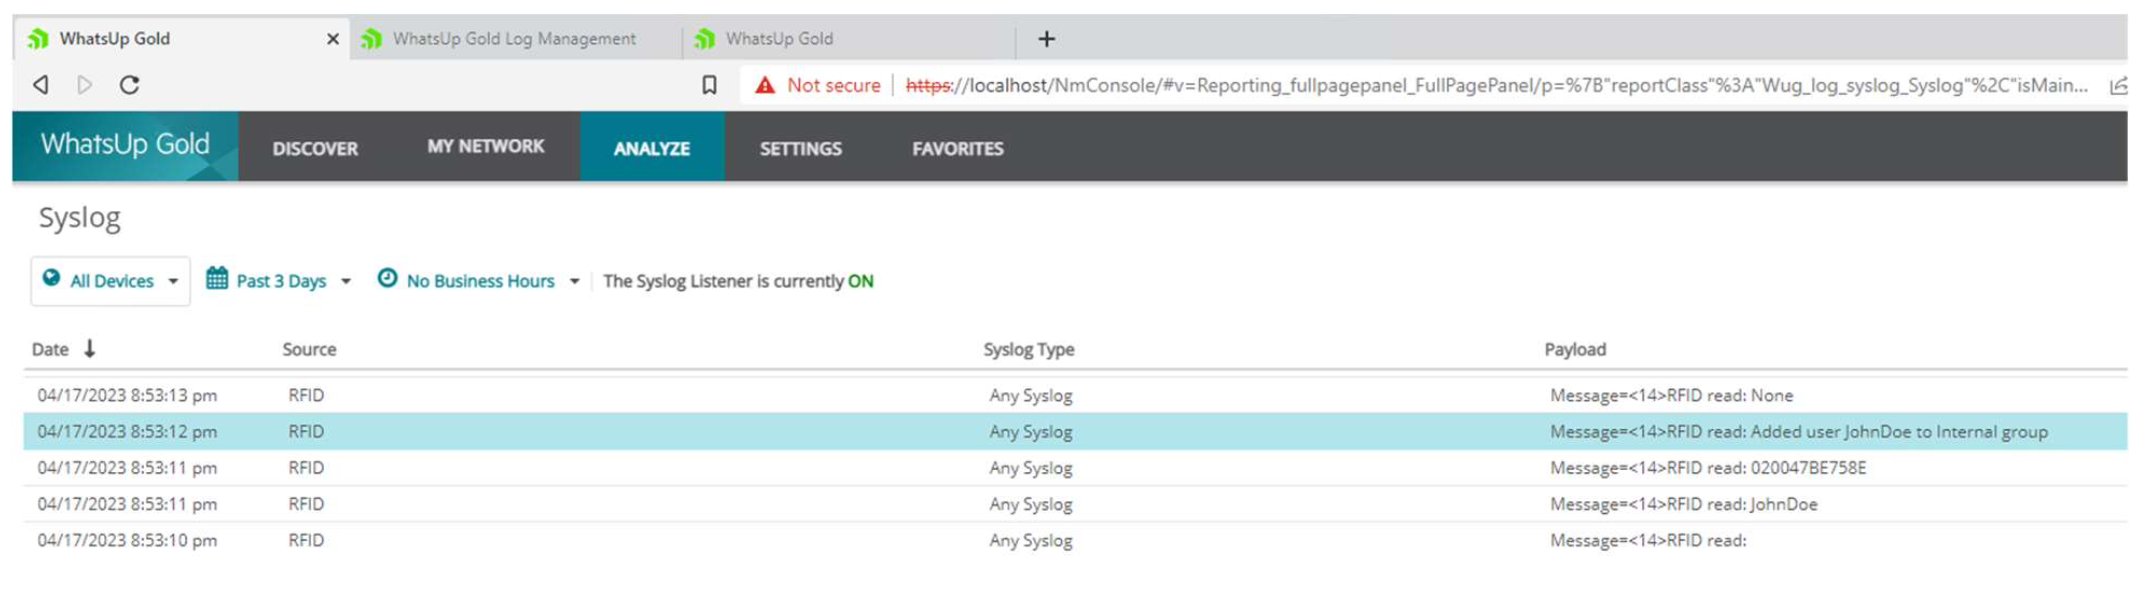
\includegraphics[width=\textwidth]{img/whatsup-gold}}
  \caption{We record all events using WhatsUp Gold.  In the above we
    observe a user changing group (from External to Internal) as they
    swipe their access card when entering a
    building.}\label{fig:whatsup-gold}
\end{figure*}

The Raspberry Pi, LM, and Flask application send logs to a SIEM
service.  We use Progress WhatsUp Gold (WUG) (see
Fig.~\ref{fig:whatsup-gold}) to gather and manage all device log data.
In normal operation the events from the Raspberry Pi, RFID door entry
system, and LM are logged.  We use the Syslog protocol, a standard
network-based logging protocol, for all events.  In cases where a
user's credentials may be compromised, the Flask application logs an
event with high priority.
